\documentclass[tikz]{standalone}
\usepackage{tikz}

\begin{document}
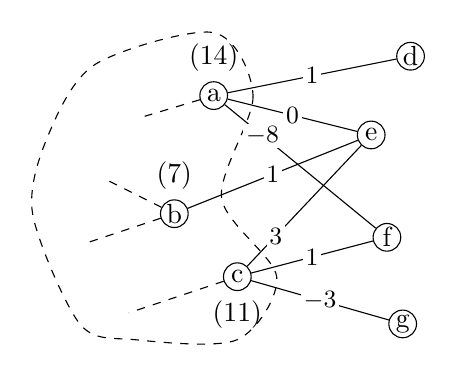
\begin{tikzpicture}
    [mynode/.style={draw,circle,inner sep = 0em, minimum size = 10},
     edgelabel/.style = {fill = white, inner sep = 1, font=\small}]
    \draw [dashed] plot [smooth cycle]
        coordinates {
            (-2.0, 1.8)
            (-1.5, 1.0)
            (-1.9, -0.3)
            (-1.2, -1.3)
            (-1.7, -2.1)
            (-3.0, -2.1)
            (-3.7, -1.9)
            (-4.3, -0.5)
            (-4.1, 0.5)
            (-3.5, 1.4)
        };

    % % draw anchor points for the curve
    % \node[mynode] at (-2.0, 1.5) {1};
    % \node[mynode] at (-1.5, 1.0) {2};
    % \node[mynode] at (-1.9, -0.3) {3};
    % \node[mynode] at (-1.2, -1.3) {4};
    % \node[mynode] at (-1.7, -2.1) {5};
    % \node[mynode] at (-3.0, -2.1) {6};
    % \node[mynode] at (-3.7, -1.9) {7};
    % \node[mynode] at (-4.3, -0.5) {8};
    % \node[mynode] at (-4.1, 0.5) {9};
    % \node[mynode] at (-3.5, 1.2) {10};

    % nodes inside the curve
    \node[mynode, label=90:{$(14)$}] (a) at (-2.0, 1) {a};
    \node[mynode, label=90:{$(7)$}] (b) at (-2.5, -0.5) {b};
    \node[mynode, label=270:{$(11)$}] (c) at (-1.7, -1.3) {c};

    % nodes outside of the curve
    \node[mynode] (d) at (0.5, 1.5) {d};
    \node[mynode] (e) at (0, 0.5) {e};
    \node[mynode] (f) at (0.2, -0.8) {f};
    \node[mynode] (g) at (0.4, -1.9) {g};

    % empty nodes and dashed edges to them
    \node (empty1) at (-3, 0.7) {};
    \node (empty2) at (-3.5, 0) {};
    \node (empty3) at (-3.2, -1.8) {};
    \node (empty4) at (-3.7, -0.9) {};
    \draw[dashed] (a) -- (empty1);
    \draw[dashed] (b) -- (empty2);
    \draw[dashed] (c) -- (empty3);
    \draw[dashed] (b) -- (empty4);

    % edges between inside and outside nodes
    \draw[-] (a) to node[edgelabel] {$1$} (d);
    \draw[-] (a) to node[edgelabel] {$0$} (e);
    \draw[-] (a) to node[edgelabel, near start] {$-8$} (f);
    \draw[-] (b) to node[edgelabel] {$1$} (e);
    \draw[-] (c) to node[edgelabel, near start] {$3$} (e);
    \draw[-] (c) to node[edgelabel] {$-3$} (g);
    \draw[-] (c) to node[edgelabel] {$1$} (f);

\end{tikzpicture}
\end{document}